\section{Experiments} 
\label{sec:experiments}
\begin{table*}[t]
	\caption{\small Comparison of performance of different models on SARCOS, MNIST and CIFAR-10. The columns ``Error (multi-path)'' and ``Error (single-path)'' indicate the classification ($\%$) or regression (MSE) errors of predictions based on the multi-path and the single-path inference. The columns ``Params. (multi-path)'' and ``Params. (single-path)'' respectively show the total number of parameters in the model and the average number of parameters used during single-path inference. ``Ensemble Size'' indicates the size of ensemble used. An entry of ``--'' indicates that no value was reported.  Methods marked with \textsuperscript{\textdagger} are from our implementations trained in the same experimental setup. * indicates that the parameters are initialised with a pre-trained CNN.}
	\label{table:mnist_results}
    \centering
    \footnotesize
	\begin{tabular}{|c|l|cc|cc|c|}
		\hline
		%\abovespace\belowspace
		& \multicolumn{1}{c|}{Method}
		& \multicolumn{1}{c}{\thead{\scriptsize Error \\ \scriptsize (multi-path)}}
		& \multicolumn{1}{c}{\thead{\scriptsize Error \\ \scriptsize (single-path)}}
		& \multicolumn{1}{c}{\thead{\scriptsize Params. \\ \scriptsize (multi-path)}}
		& \multicolumn{1}{c|}{\thead{\scriptsize Params. \\ \scriptsize (single-path)}}
		& \multicolumn{1}{c|}{\thead{\scriptsize Ensemble \\ \scriptsize Size}} \\	
		\hline
		\parbox[t]{2mm}{\multirow{12}{*}{\rotatebox[origin=c]{90}{SARCOS}}}
		& Linear regression & 10.693 & N/A & 154 & N/A & 1 \\
		& MLP with 2 hidden layers \cite{zhao2017efficient} & 5.111 & N/A & 31,804 & N/A & 1 \\
		& Decision tree & 3.708 & 3.708 & 319,591 & 25 & 1 \\
		& MLP with 1 hidden layer & 2.835 & N/A & 7,431 & N/A & 1 \\
		& Gradient boosted trees & 2.661 & 2.661 & 391,324 & 2,083 & 7 $\times$ 30 \\
		& MLP with 5 hidden layers & 2.657 & N/A & 270,599 & N/A & 1 \\
		& Random forest & 2.426 & 2.426 & 40,436,840 & 4,791 & 200 \\
		& Random forest & 2.394 & 2.394 & 141,540,436 & 16,771 & 700 \\
		& MLP with 3 hidden layers & 2.129 & N/A & 139,015 & N/A & 1 \\
		&\cellcolor{gray!10}SDT (with MLP routers) &\cellcolor{gray!10} 2.118 &\cellcolor{gray!10} 2.246 &\cellcolor{gray!10} 28,045  &\cellcolor{gray!10} 10,167 &\cellcolor{gray!10} 1\\
		& Gradient boosted trees & 1.444 & 1.444 & 988,256 & 6,808 & 7 $\times$ 100 \\
		&\cellcolor{gray!10}ANT-SARCOS &\cellcolor{gray!10} 1.384 &\cellcolor{gray!10}  1.542 &\cellcolor{gray!10} 103,823  
		&\cellcolor{gray!10} 61,640 &\cellcolor{gray!10} 1\\
		&\cellcolor{gray!10}ANT-SARCOS (ensemble) &\cellcolor{gray!10} 1.226 &\cellcolor{gray!10}  1.372 &\cellcolor{gray!10} 598,280  
		&\cellcolor{gray!10} 360,766 &\cellcolor{gray!10} 8\\
		\hline
		%\abovespace
		\parbox[t]{2mm}{\multirow{14}{*}{\rotatebox[origin=c]{90}{MNIST}}}
        & Linear classifier & 7.91& N/A & 7,840 & N/A&1\\
        & RDT \cite{leon2015policy} & 5.41 & --~~~ & --~~~ & --~~~ & 1\\
		& Random Forests \cite{breiman2001random}& 3.21 & 3.21 & --~~~ & --~~~ &200\\
        & Compact Multi-Class Boosted Trees \cite{ponomareva2017compact} & 2.88 & -- & --~~~  & --~~~ &100 \\
		& Alternating Decision Forest  \cite{schulter2013alternating} & 2.71 & 2.71 & --~~~  & --~~~ &20 \\
		& Neural Decision Tree \cite{xiao2017ndt}& 2.10 & --~~~ &1,773,130 & 502,170&1\\
		&\cellcolor{gray!10}ANT-MNIST-C &\cellcolor{gray!10} 1.62 &\cellcolor{gray!10} 1.68 &\cellcolor{gray!10} 39,670 &\cellcolor{gray!10} 7,956 &\cellcolor{gray!10} 1\\
		& MLP with 2 hidden layers \cite{simard2003best}& 1.40 & N/A & 1,275,200& N/A&1 \\
        & LeNet-5\textsuperscript{\textdagger} \cite{lecun1998gradient} & 0.82 & N/A& 431,000 & N/A & 1\\
		& gcForest \cite{zhou2017deepft} & 0.74 &  0.74 & --~~~  & --~~~  & 500\\
		&\cellcolor{gray!10}ANT-MNIST-B &\cellcolor{gray!10} 0.72 &\cellcolor{gray!10} 0.73 &\cellcolor{gray!10} 76,703 &\cellcolor{gray!10} 50,653 &\cellcolor{gray!10} 1\\
		& Neural Decision Forest \cite{kontschieder2015deep} & 0.70 & --~~ & 544,600 & 463,180 & 10\\
		&\cellcolor{gray!10}ANT-MNIST-A &\cellcolor{gray!10} 0.64 &\cellcolor{gray!10} 0.69 &\cellcolor{gray!10} 100,596&\cellcolor{gray!10} 84,935 &\cellcolor{gray!10} 1\\
		&\cellcolor{gray!10}ANT-MNIST-A (ensemble) &\cellcolor{gray!10} 0.29 &\cellcolor{gray!10} 0.30 &\cellcolor{gray!10} 850,775 &\cellcolor{gray!10} 655,449 &\cellcolor{gray!10} 8 \\
		%		\rowcolor{gray!10} \cellcolor{white} &ANT-MNIST-1 & 0.64 & 0.69 & 100,596& 94,935 & 1\\
		%		\rowcolor{gray!10} \cellcolor{white} &ANT-MNIST-2 & 0.72 & 0.73 &  76,703 & 60,653 & 1\\
		%		\rowcolor{gray!10} \cellcolor{white} &ANT-MNIST-6 & 1.62 & 1.68&  39,670 & 7,956 & 1\\
        & CapsNet \cite{sabour2017dynamic} & 0.25 & --~~ & 8.2M & N/A & 1\\
		\hline
		%\abovespace
		\parbox[t]{2mm}{\multirow{13}{*}{\rotatebox[origin=c]{90}{CIFAR-10}}}                
        & Compact Multi-Class Boosted Trees \cite{ponomareva2017compact} & 52.31 & -- & --~~~  & --~~~ &100 \\
        & Random Forests  \cite{breiman2001random}& 50.17 & 50.17 & --~~~ & --~~~ &2000\\
		& gcForest \cite{zhou2017deepft} & 38.22&  38.22 & --~~~  & --~~~  & 500\\
		& MaxOut \cite{goodfellow2013maxout} & 9.38 & N/A& 6M & N/A & 1\\
        &\cellcolor{gray!10}ANT-CIFAR10-C & \cellcolor{gray!10}9.31 & \cellcolor{gray!10}  9.34& \cellcolor{gray!10} 0.7M &\cellcolor{gray!10} 0.5M & \cellcolor{gray!10}1\\
        &\cellcolor{gray!10}ANT-CIFAR10-B & \cellcolor{gray!10}9.15 & \cellcolor{gray!10}  9.18&  \cellcolor{gray!10}0.9M &\cellcolor{gray!10}0.6M& \cellcolor{gray!10}1\\
		%& dasNet (Stolenga et al., 2014) & 9.22 & N/A & 6M& N/A&1 \\
		& Network in Network \cite{lin2013network} & 8.81 & N/A & 1M  &N/A &1 \\
		& All-CNN\textsuperscript{\textdagger}\cite{springenberg2014striving} & 8.71 & N/A & 1.4M  & N/A &1 \\
		&\cellcolor{gray!10}ANT-CIFAR10-A & \cellcolor{gray!10}8.31 & \cellcolor{gray!10}  8.32 &\cellcolor{gray!10}1.4M&\cellcolor{gray!10}1.0M & \cellcolor{gray!10}1\\
		&\cellcolor{gray!10}ANT-CIFAR10-A (ensemble) & \cellcolor{gray!10}7.71 & \cellcolor{gray!10}  7.79 &\cellcolor{gray!10}8.7M&\cellcolor{gray!10}7.4M & \cellcolor{gray!10}8\\
		&\cellcolor{gray!10}ANT-CIFAR10-A* & \cellcolor{gray!10}6.72 & \cellcolor{gray!10} 6.74 &\cellcolor{gray!10}1.3M&\cellcolor{gray!10}0.8M & \cellcolor{gray!10}1\\
        & ResNet-110 \cite{he2016deep} & 6.43 & N/A & 1.7M  &N/A &1 \\
        & DenseNet-BC (k=24) \cite{huang2017densely} & 3.74 & N/A & 27.2M  &N/A &1 \\
		\hline
		\end{tabular}
\end{table*}

We evaluate ANTs using the SARCOS multivariate regression dataset \cite{vijayakumar2000locally}, and the MNIST \cite{lecun1998gradient} and CIFAR-10 \cite{krizhevsky2009learning} classification datasets. We run ablation studies to show that our different components are vital for the best performance. We then assess the ability of ANTs to automatically learn meaningful hierarchical structures in data. Next, we examine the effects of refinement phase on ANTs, and show that it can automatically prune the tree. Finally, we demonstrate that our proposed training procedure adapts the model size appropriately under varying amounts of labelled data. All of our models are implemented in PyTorch \cite{paszke2017automatic} and is available at  \url{https://github.com/rtanno21609/AdaptiveNeuralTrees}. Full training details, including training times, are provided in Supp.~Sec.~C and D.
% \vspace{-2mm}
% \subsection{Set-up}
% \vspace{-2mm}
% We train ANTs with a range of primitive modules as shown in Tab. \ref{table:modules}. For simplicity, we define the modules based on three types of NN layers: convolutional, global-average-pooling (GAP) and fully-connected (FC). Solver modules are fixed as linear models e.g. logistic regression and linear regression. Router modules are binary classifiers with a sigmoid output. All convolutional and FC layer are followed by ReLU or tanh non-linearities, except in the last layers of solvers and routers. We also apply $2\times2$ max-pooling to feature maps after every $d$ transformer modules where $d$ is the downsample frequency. For the regression experiment, hidden layers in the baseline MLPs, routers and transformers contain 256 units. We balance the number of parameters in the router and transformer modules to be of the same order of magnitude to avoid favouring either partitioning the data or learning more expressive features. In the growth phase the parameters for the new modules are trained until convergence, as determined by patience-based early stopping on the validation set. The patience level is an important hyperparameter tuned based on the validation set, and a quantitative evaluation of its effect on performance is given in Supp.~Sec.~E. Full training details, including training times, are provided in Supp.~Sec.~C and D, with details of ANT ensembles provided in Supp.~Sec.~I.

\subsection{Model Performance}
We compare the performance of ANTs (Tab. \ref{table:modules}) against a range of DT and NN models (Tab. \ref{table:mnist_results}), where notably the relative performance of these two classes of models differs between datasets. ANTs inherit from both and achieve the lowest error on SARCOS, and perform favourably on MNIST and CIFAR-10. In general, DT methods without feature learning, such as RFs \cite{breiman2001random,zhou2017deepft} and GBTs \cite{ponomareva2017compact}, perform poorly on image classification tasks \cite{krizhevsky2009learning}. In comparison with CNNs without shortcut connections \cite{lecun1998gradient,goodfellow2013maxout,lin2013network,springenberg2014striving}, different ANTs balance between stronger performance with comparable numbers of trainable parameters, and comparable performance with smaller amount of parameters. At the other end of the spectrum, state-of-the-art NNs \cite{sabour2017dynamic,huang2017densely} contain significantly more parameters.
%On these image datasets, ANTs outperform other NNs with similar parameter counts, but fail to reach the performance of state-of-the-art models \cite{sabour2017dynamic,huang2017densely} which contain an order of magnitude more parameters.

\textbf{Conditional computation:} Tab.\ref{table:mnist_results} compares the errors and number of parameters of different ANTs for both multi-path and single-path inference schemes. While reducing the number of parameters (from Params (multi-path) to Params (single-path)) across all ANT models, we observe only a small difference in error (between Error (multi-path) and Error (single-path)), with the largest deviations being $0.06\%$ for classification and $0.158$ for regression. In addition, Supp.Sec.~H shows that the single-path inference reduces FLOPS. This means that single-path inference gives an accurate approximation of the multi-path inference, while being more efficient to compute. This close approximation comes from the confident splitting probabilities of routers, being close to 0 or 1 (see blue histograms in Fig. \ref{fig:learnedmodel}(b)).

% The latter would, however, require computing the probabilities of reaching all the nodes of the tree, which engages all operational modules except the solvers and thus is almost as expensive as computing the full distribution. We therefore instead approximate the most confident path by traversing the tree in the directions of higher confidence of routers. This approximation allowes us to constrain the computation to a single path and holds true in most cases (error rate $0.01\%$) as the router modules guide data points with high confidence.

% \textbf{Patience-based local optimisation:} in the growth phase the parameters for the new modules are trained until convergence, as determined by patience-based early stopping on the validation set. We observe that very low or high patience levels result in new modules underfitting or overfitting locally, thus preventing meaningful further growth% and leading to differences of up to 10\% in validation accuracy.
% . We tuned this hyperparameter using the validation sets, and set the patience level to $5$, which produced consistently good performance on both MNIST and CIFAR-10 datasets across different specifications of primitive modules. A quantitative evaluation is given in the supplementary (Sec.~E).

%in the growth phase, the number of optimisation steps spent for the trial of each new model affects the discovered architecture, and consequently the classification performance. If too few steps of optimisation are performed, then the added modules would not be tuned enough. On the other hand, if too many optimisation steps are taken, this causes the added component to overfit locally. Both extremes prevent the model from making a meaningful further growth. We thus employed patience based early-stopping, and selected the best patience level based on validation accuracy on both MNIST and CIFAR-10. A quantitative evaluation is given in the supplementals.
\textbf{Ablation study:} we compare the predictive errors of different variants of ANTs in cases where the options for adding transformer or router modules are disabled (see Tab. \ref{tab:ablationstudy}). In the first case, the resulting models are equivalent to SDTs \cite{suarez1999globally} or HMEs \cite{jordan1994hierarchical} with locally grown architectures, while the second case is equivalent to standard CNNs, grown adaptively layer by layer. We observe that either ablation consistently leads to higher errors across different module configurations on all three datasets, justifying the combination of feature learning and hierarchical partitioning in ANTs.

\textbf{SARCOS multivariate regression:} Tab.~\ref{table:mnist_results} shows that ANT-SARCOS outperforms all other methods in mean squared error (MSE) with the full set of parameters. With the single-path inference, GBTs performs slightly better than a single ANT while requiring fewer parameters. We note that the top 3 methods are all tree-based, with the third best method being an SDT (with MLP routers). On the other hand, ANT and GBTs outperform the best standard NN model with less than a half of the parameter count. This highlights the value of hierarchical clustering for predictive performance and inference speed. Meanwhile, we still reap the benefits of representation learning, as shown by both ANT-SARCOS and the SDT (which is a specific form of ANT with identity transformers) requiring fewer parameters than the best-performing GBT configuration. Finally, we note that deeper NNs (5 vs. 3 hidden layers) can overfit on this small dataset, which makes the adaptive growth procedure of tree-based methods ideal for finding a model that exhibits good generalisation. 



%Tab.~\ref{table:mnist_results} shows that ANT-SARCOS outperforms all other methods in mean squared error (MSE) with the full set of parameters. With the single-path inference, GBTs performs slightly better than a single ANT while requiring fewer parameters. An ensemble of ANTs achieves the best results over all in both multi- and single-path inference. We note that the top 3 performing methods are all tree-based, with the third best method being an SDT (with MLP routers). %Despite the proliferation of deep-learning-based methods for highly structured data such as images and text, GBTs and RFs can still outperform them on other sorts of data, such as we have here. 
%This highlights the value of hierarchical clustering of the input space for predictive performance. Meanwhile, we still reap the benefits of representation learning, as shown by both ANT-SARCOS and the SDT (which is a specific form of ANT with identity transformers) requiring fewer parameters than the best-performing GBT configuration. Finally, we note that deeper NNs (5 vs. 3 hidden layers) can overfit on this small dataset, which makes the adaptive growth procedure of tree-based methods ideal for finding a model that exhibits good generalisation.

%Tab.~\ref{table:mnist_results} shows that the top 3 models are all tree-based, with NDT, GBTs and ANT achieving the lowest MSE. ANT requires less than a half of what’s required for the best standard NN model. On the other hand, Gradient Boosted trees only need a magnitude less parameters. We should however note that the total number of parameters for standard trees models are significantly larger than that of an ANT. All in all, ANT achieves the best accuracy on SARCOS beating both standard NNs and standard tree-based methods. Secondly, in terms of computational efficiency, ANTs is somewhere between NNs and GBTs. This highlights the value of hierarchical clustering of the input space for both predictive accuracy and speed. 

\textbf{MNIST digit classification:} we observe that ANT-MNIST-A outperforms state-of-the-art GBT \cite{ponomareva2017compact} and RF \cite{zhou2017deepft} methods in accuracy. This performance is attained despite the use of a single tree, while RF methods operate with ensembles of classifiers (the size shown in Tab. \ref{table:modules}). In particular, the NDF \cite{kontschieder2015deep} has a pre-specified architecture where LeNet-5 \cite{lecun1998gradient} is used as the root transformer module, and $10$ trees of fixed depth $5$ are built on this base features. On the other hand, ANT-MNIST-A is constructed in a data-driven manner from primitive modules, and displays an improvement over the NDF both in terms of accuracy and number of parameters. In addition, reducing the size of convolution kernels (ANT-MNIST-B) reduces the total number of parameters by $25\%$ and the path-wise average by almost $40\%$ while only increasing the error by $< 0.1\%$.

We also compare against the LeNet-5 CNN \cite{lecun1998gradient}, comprised of the same types of operations used in our primitive modules (i.e. convolutional, max-pooling and FC layers). For a fair comparison, the network is trained with the same protocol as that of the ANT refinement phase, achieving an error rate of $0.82\%$. Both ANT-MNIST-A and ANT-MNIST-B attain better accuracy with a smaller number of parameters than LeNet-5. The current state-of-the-art, capsule networks (CapsNets) \cite{sabour2017dynamic}, have more parameters than ANT-MNIST-A by almost two orders of magnitude.\footnote{Notably, CapsNets also feature a routing mechanism, but with a significantly different mechanism and motivation.} By ensembling ANTs, we can reach similar performance ($0.29\%$ versus $0.25\%$) with an order of magnitude less parameters (see Supp.Sec.~H).

Lastly, we highlight the observation that ANT-MNIST-C, with the simplest primitive modules, achieves an error rate of $1.68\%$ with single-path inference, which is significantly better than that of the linear classifier ($7.91\%$), while engaging almost the same number of parameters ($7,956$ vs. $7,840$) on average. To isolate the benefit of convolutions, we took one of the root-to-path CNNs on ANT-MNIST-C and increased the number of kernels to adjust the number of parameters to the same value. We observe a higher error rate of $3.55\%$, which indicates that while convolutions are beneficial, data partitioning has additional benefits in improving accuracy. This result demonstrates the potential of ANT growth protocol for constructing performant models with lightweight inference. See Sec.~G in the supplementary materials for the architecture of ANT-MNIST-C.

\begin{table}[t]
	\caption{\footnotesize Ablation study on regression (MSE) and classification ($\%$) errors. ``CNN'' refers to the case where the ANT is grown without routers while ``SDT/HME'' refers to the case where transformer modules on the edges are disabled.} \label{tab:ablationstudy}
	\footnotesize
    \center
	\begin{tabular}{|l|ccc|ccc|}
		\hline
		\multicolumn{1}{|c}{\textbf{Model}} &  \multicolumn{3}{|c|}{\textbf{Error (multi-path)}} & \multicolumn{3}{c|}{\textbf{Error (single-path)}}  \\
			& ANT & CNN & HME & ANT & CNN & HME  \\
			& (default) & (no $\mathcal{R}$) & (no $\mathcal{T}$) & (default) & (no $\mathcal{R}$) & (no $\mathcal{T}$) \\
		\hline
		SARCOS &1.38 & 2.51 & 2.12 &1.54 & 2.51 & 2.25 \\
		MNIST-A &0.64 & 0.74 & 3.18 &0.69 & 0.74 & 4.19  \\
	    MNIST-B &0.72 & 0.80 & 4.63 &0.73 & 0.80 & 3.62\\
        MNIST-C &1.62 & 3.71 & 5.70 &1.68 & 3.71 & 6.96 \\
		CIFAR10-A &8.31 & 9.29 & 39.29   & 8.32 & 9.29 & 40.33 \\
        CIFAR10-B &9.15 & 11.08 & 43.09 & 9.18 & 11.08 & 44.25 \\
        CIFAR10-C &9.31 & 11.61 & 48.59 & 9.34 & 11.61 & 50.02 \\
		\hline
	\end{tabular}
\end{table}

\textbf{CIFAR-10 object recognition:} we see that ANTs largely outperform the state-of-the-art DT method, gcForest \cite{zhou2017deepft}, achieving over 90\% accuracy, demonstrating the benefit of representation learning in tree-structured models. Secondly, with fewer number of parameters in single-path inference, ANT-CIFAR-A achieves higher accuracy than CNN models without shortcut connections \cite{goodfellow2013maxout,lin2013network,springenberg2014striving} that held the state-of-the-art performance in respective years. With simpler primitive modules we learn more compact models (ANT-MNIST-B and -C) with a marginal compromise in accuracy. In addition, initialising the parameters of transformers and routers from a pre-trained single-path CNN further reduced the error rate of ANT-MNIST-A by 20\% (see ANT-MNIST-A* in Tab. \ref{table:mnist_results}), indicating room for improvement in our proposed optimisation method.

Shortcut connections \cite{fahlman1990cascade} have recently lead to leaps in performance in deep CNNs \cite{he2016deep,huang2017densely}. We observe that our best network, ANT-MNIST-A*, has a comparable error rate and half the parameter count (with single-path inference) to the best-performing residual network, ResNet-110 \cite{he2016deep}. Densely connected networks leads to better accuracy, but with an order of magnitude more parameters \cite{huang2017densely}. We expect shortcut connections to improve ANT performance, and leave integrating them to future work.

%We note that the comparison is limited to NNs of up to 15 layers with same set of operations (e.g. convolutions, GAP and FC layers) and linear architectures. For simplicity, we did not consider primitive modules based on more recent models such as residual \cite{he2016deep} and dense connections \cite{huang2017densely}, which present lower error rates than our best result. However, ANTs are ameable to these advances.

%\textcolor{red}{we compare variants of ANTs with module specifications in Tab. \ref{table:modules} against modern NN models, and results are summarized in the bottom half of Tab.\ref{table:mnist_results}. We limit our comparison to NNs of up to $15$ layers with the same set of simple operations and linear architectures. In particular, we choose All-CNN as the baseline which reports the lowest error among the comparison targets and is the closest in terms of constituent operations (convolutional, GAP and FC layers). For a fair comparison, we train our reimplementation of the model in the same experimental set-up as the refinement phase of ANT training, and report the new performance. We also apply batch normalization \cite{ioffe2015batch} after every convolutional layer both in ANT modules, and All-CNN, as it improved convergence and accuracy.} We observe that our growth protocol can discover an architecture (ANT-CIFAR10-A) which attains lower error than All-CNN while retaining a similar number of parameters in total, and $20\%$ less for path-wise inference. Simpler modules lead to more compact models (ANT-CIFAR10-B and C) with a marginal compromise in accuracy.
%\textcolor{blue}{It should be noted that our framework is amenable to more recent advances in deep learning, such as residual learning \cite{he2016deep} and dense connections \cite{huang2017densely}, which all present lower error rates than our best result, but can also be integrated into ANT modules. We leave an investigation of these more complex “primitives” for future work.}

%\subsection{Learned hierarchical structures}
\subsection{Interpretability}
The growth procedure of ANTs is capable of discovering hierarchical structures in the data that are useful to the end task. Without any regularization imposed on routers, the learned hierarchies often display strong specialisation of paths to certain classes or categories of data on both the MNIST and CIFAR-10 datasets. Fig. \ref{fig:learnedmodel} (a) displays an example with particularly ``human-interpretable'' partitions e.g. man-made versus natural objects, and road vehicles versus other types of vehicles. It should, however, be noted that human intuitions on relevant hierarchical structures do not necessarily equate to optimal representations, particularly as datasets may not necessarily have an underlying hierarchical structure, e.g., MNIST. Rather, what needs to be highlighted is the ability of ANTs to learn when to share or separate the representation of data to optimise end-task performance, which gives rise to automatically discovering such hierarchies. To further attest that the model learns a meaningful routing strategy, we also present the test accuracy of the predictions from the leaf node with the smallest reaching probability in Supp.~Sec.~F. We observe that using the least likely ``expert'' leads to a substantial drop in classification accuracy. In addition, most learned trees are unbalanced. This property of adaptive computation is plausible since certain types of images may be easier to classify than others, as seen in prior work \cite{Figurnov2017SpatiallyAC}.

\subsection{Effect of global refinement} \label{sec:refinement}
\begin{figure*}[t!]
	\center
	\begin{subfigure}[t]{0.9\linewidth}
		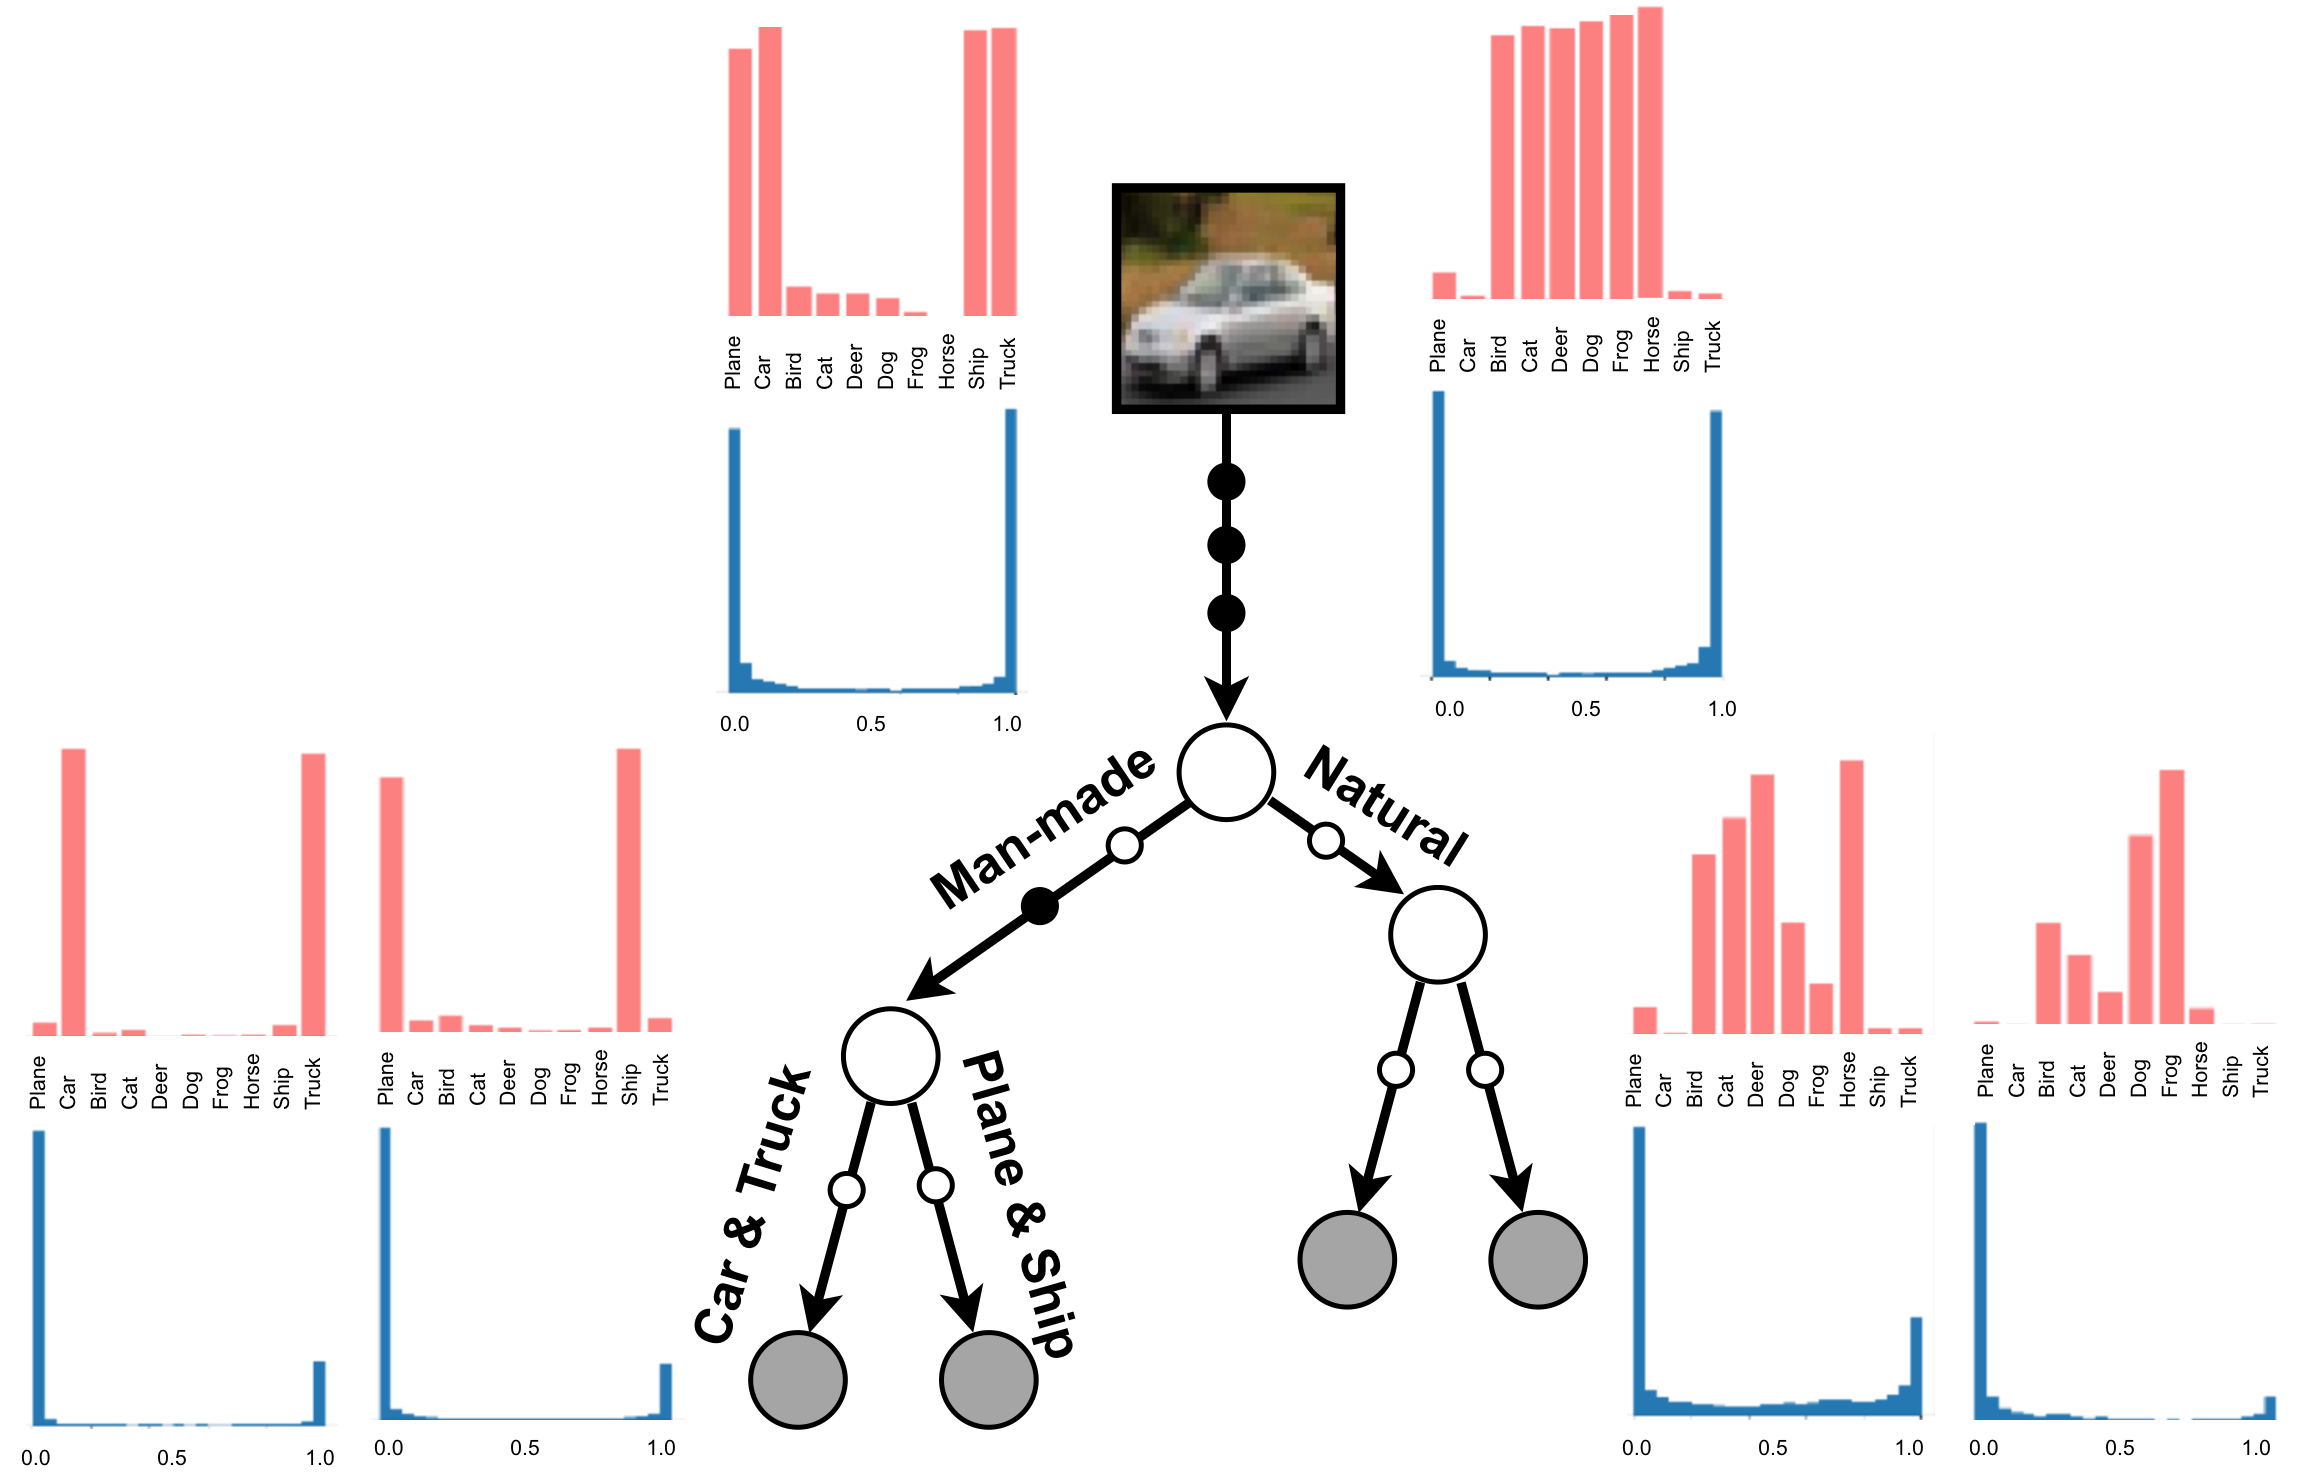
\includegraphics[width=\linewidth]{chapter_7/figures/fig_7_9.png}
		%\label{fig:ch5:active}
		\vspace{-6mm}
		\caption{Before refinement}
	\end{subfigure}
	\hspace{4.66mm}
	\begin{subfigure}[t]{0.9\linewidth}
		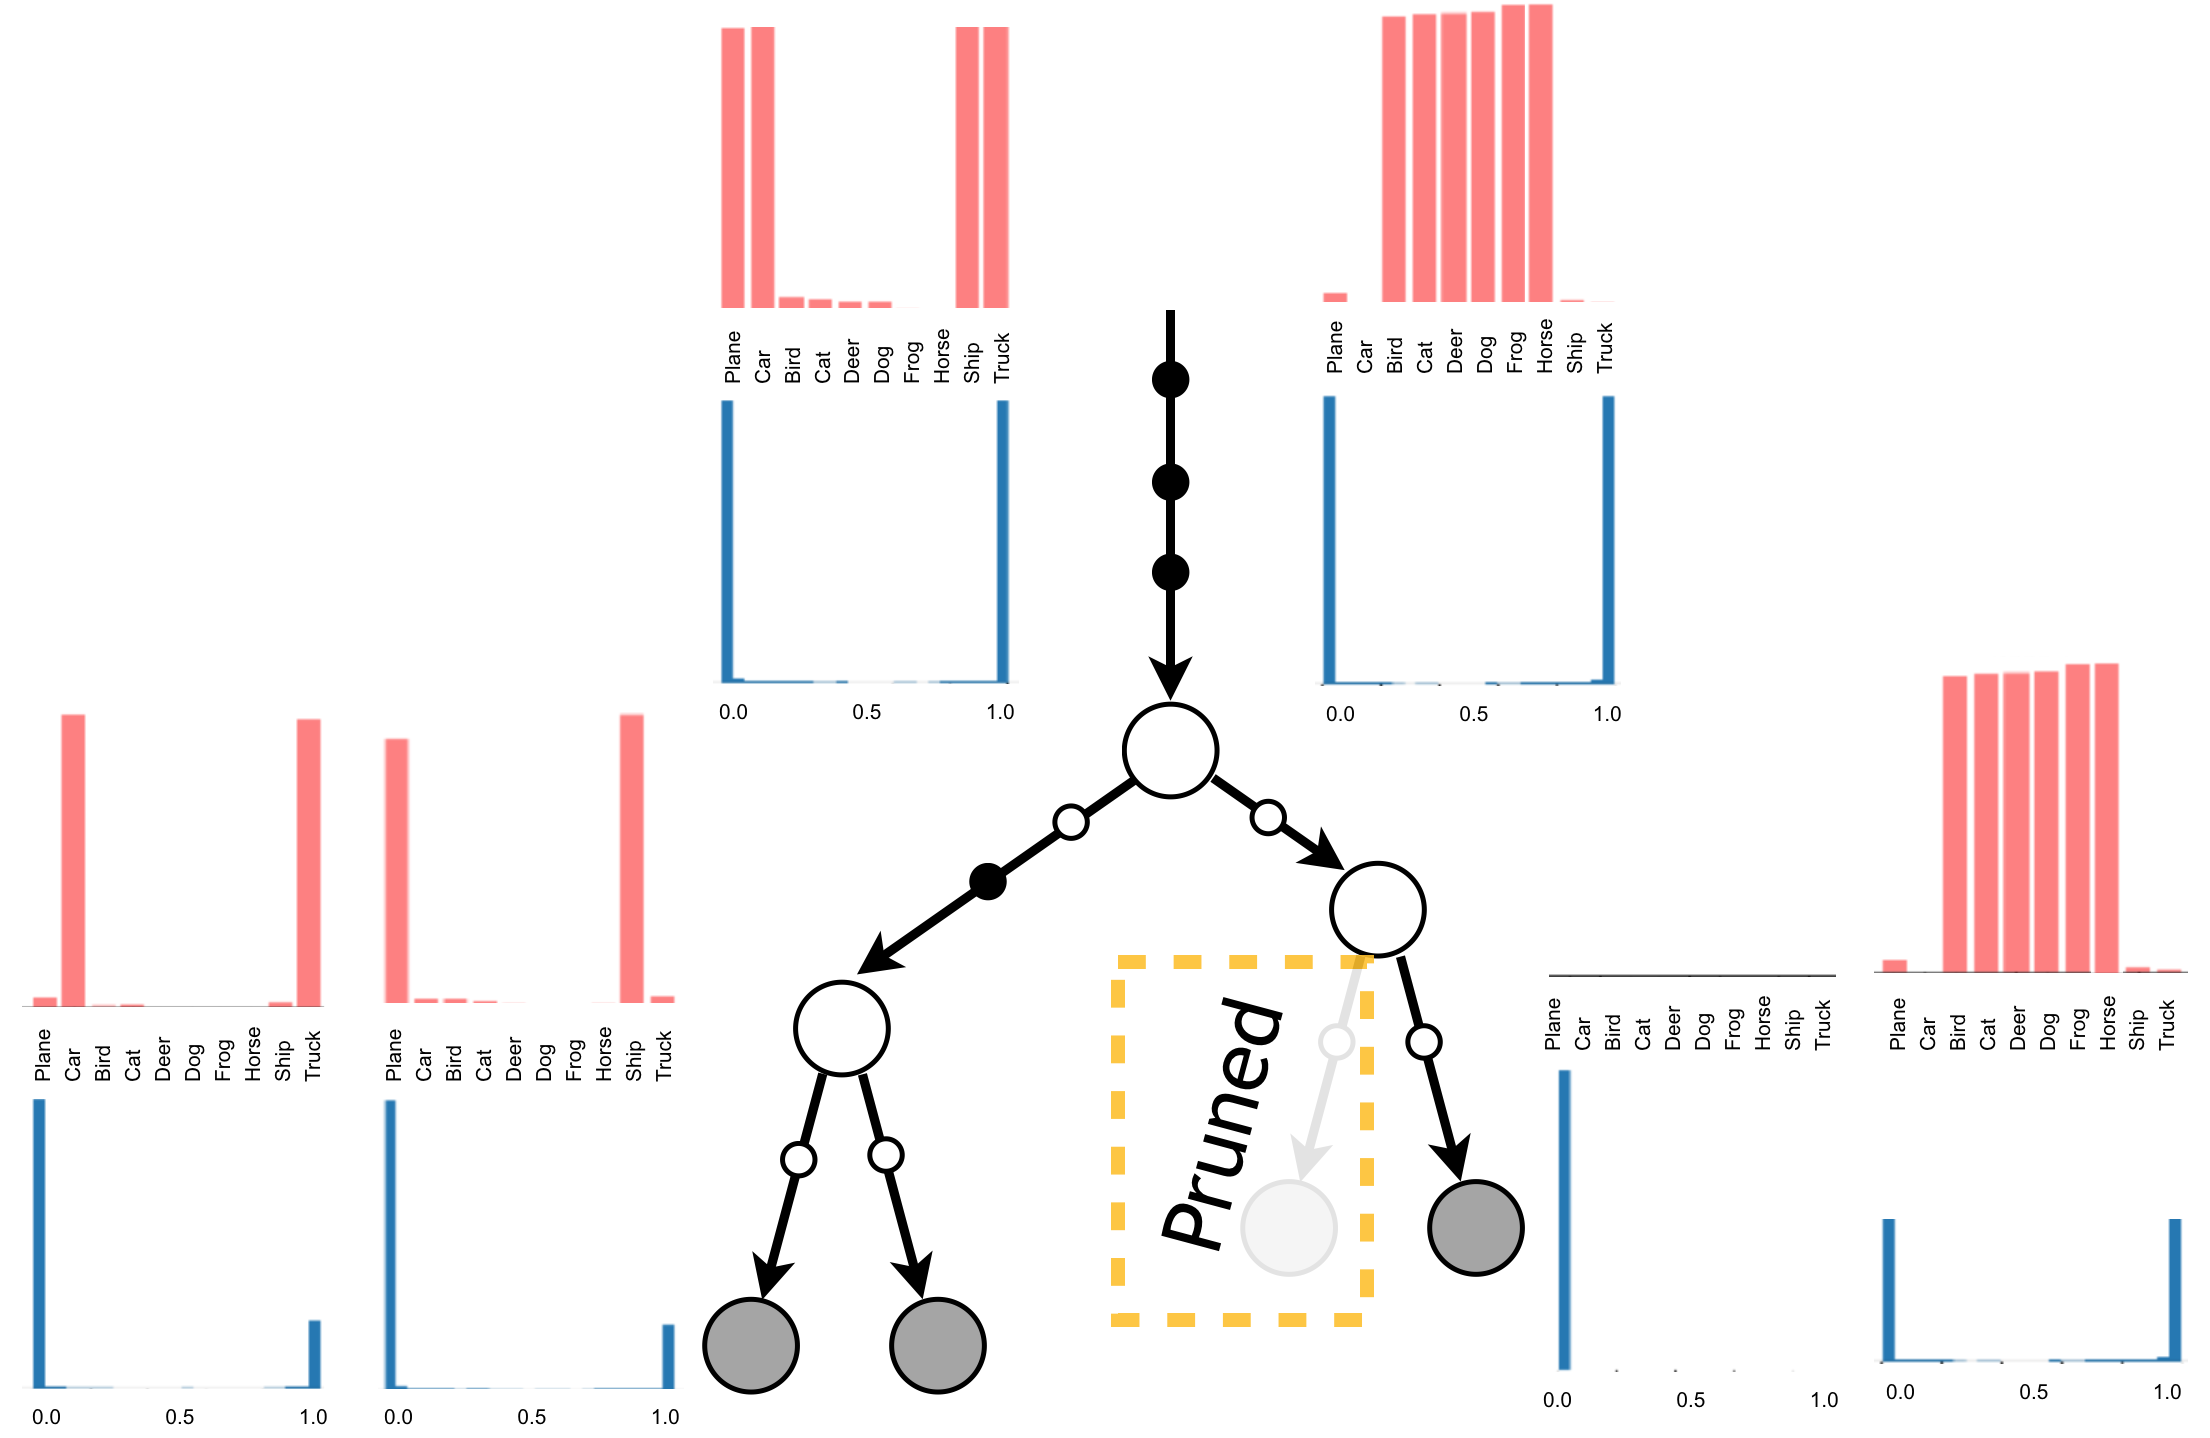
\includegraphics[width=\linewidth]{chapter_7/figures/fig_7_10.png}
		%\label{fig:ch5:active2}
		\vspace{-6mm}
		\caption{After refinement}
	\end{subfigure}
	\caption{\small Visualisation of class distributions (red) and path probabilities (blue) computed over the whole test set at respective nodes of an example ANT (a) before and (b) after the refinement phase. (a) shows that the model captures an interpretable hierarchy, grouping semantically similar images on the same branches. (b) shows that the refinement phase polarises path probabilities, pruning a branch.}
	\label{fig:learnedmodel}
\end{figure*}

\begin{figure}[t!]
	\centering
	\begin{subfigure}[t]{0.48\linewidth}
		\caption{}
		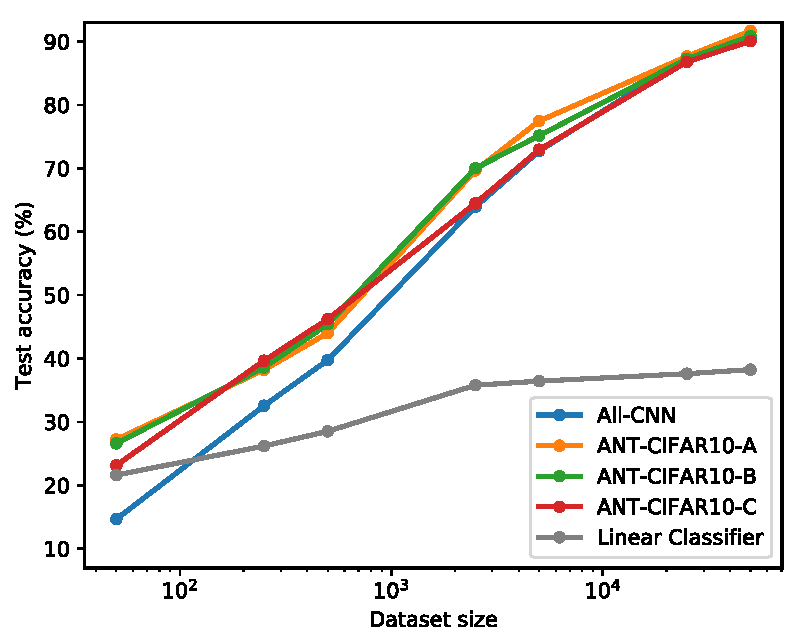
\includegraphics[width=\linewidth]{chapter_7/figures/fig_1_2.pdf}
		%\label{fig:ch5:active}
	\end{subfigure}
	\hspace{0mm}
	\begin{subfigure}[t]{0.50\linewidth}
		\caption{}
		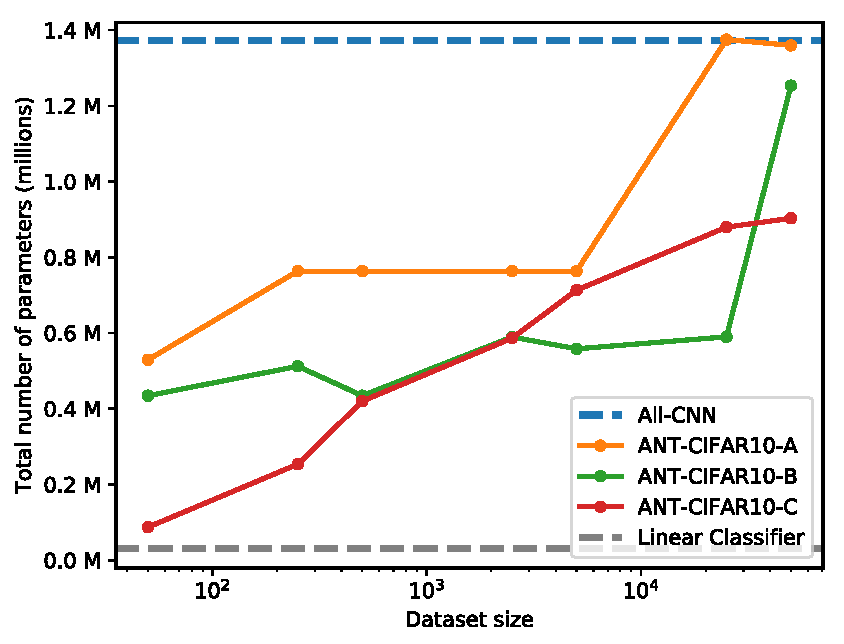
\includegraphics[width=\linewidth]{chapter_7/figures/fig_2_2.pdf}
		%\label{fig:ch5:active2}
	\end{subfigure}
	\hspace{0mm}
	\begin{subfigure}[t]{0.52\linewidth}
		\caption{}
		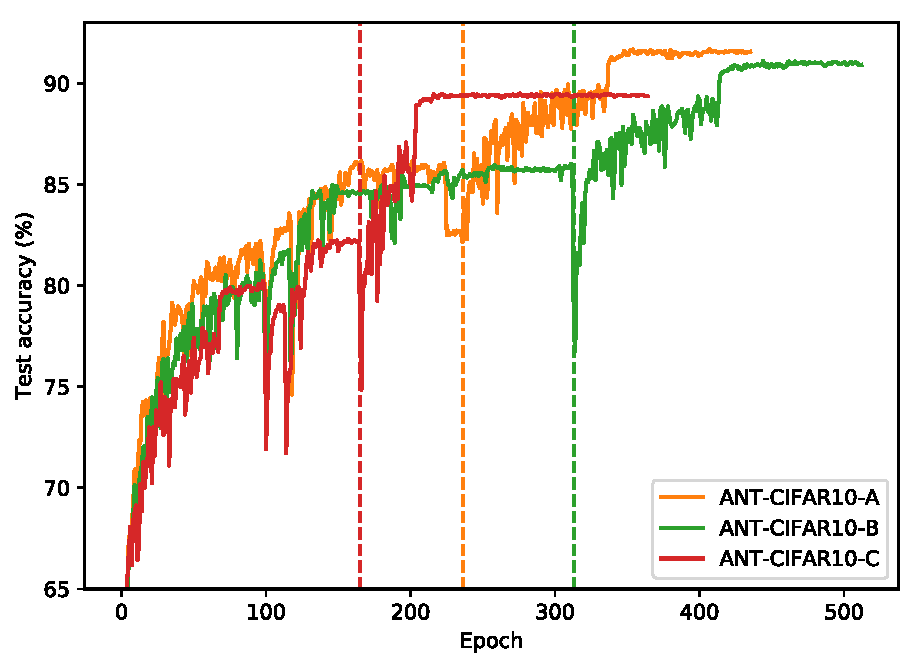
\includegraphics[width=\linewidth]{chapter_7/figures/fig_3_2.pdf}
		%\label{fig:ch5:active2}
	\end{subfigure}
	\caption{\small (a) Test accuracy on CIFAR-10 of ANTs for varying amounts of training data. (b) The complexity of the grown ANTs increases with dataset size. (c) Refinement improves generalisation; the dotted lines show where the refinement phase starts.}
	\label{fig:cifar10}
\end{figure}

We observe that global refinement phase improves the generalisation error. Fig. \ref{fig:cifar10} (Right) shows the generalisation error of various ANT models on CIFAR-10, with vertical dotted lines indicating the epoch when the models enter the refinement phase. As we switch from optimising parts of the ANT in isolation to optimising all parameters, we shift the optimisation landscape, resulting in an initial drop in performance. However, they all consistently converge to higher test accuracy than the best value attained during the growth phase. This provides evidence that refinement phase remedies suboptimal decisions made during the locally-optimised growth phase. In many cases, we observed that global optimisation polarises the decision probability of routers, which occasionally leads to the effective ``pruning" of some branches. For example, in the case of the tree shown in Fig. \ref{fig:learnedmodel}(b), we observe that the decision probability of routers are more concentrated near 0 or 1 after global refinement, and as a result, the empirical probability of visiting one of the leaf nodes, calculated over the validation set, reduces to 0.09\%---meaning that the corresponding branch could be pruned without a negligible change in the network's accuracy. The resultant model attains lower generalisation error, showing the pruning has resolved a suboptimal partioning of data. 
%We emphasise that this is a consequence of global fine-tuning, and does not involve additional algorithms that would be used to prune or compress standard NNs.

%We observe that global refinement step improves the generalisation error. Fig. \ref{fig:cifar10} (right) shows the generalisation error on CIFAR-10 of various ANT models, with vertical dotted lines indicating the epoch when the models enter the refinement phase. While the models initially undergo a steep drop in performance, they all consistently converge to higher test accuracy than the best value attained during the growth phase. This provides evidence that global optimisation remedies suboptimal decisions made during the locally optimised growth phase. For example, refinement tends to polarize the decisions of routers, which can allow some branches to be pruned (see Fig. \ref{fig:learnedmodel}); this improves generalisation, indicating resolvement of suboptimal partitioning of data. 


\subsection{Adaptive model complexity}
Overparametrised models, trained without regularization, are vulnerable to overfitting on small datasets. Here we assess the ability of our proposed ANT training method to adapt the model complexity to varying amounts of labelled data. We run classfication experiments on CIFAR-10 and train three variants of ANTs, All-CNN \cite{springenberg2014striving} and linear classifier on subsets of the dataset of sizes 50, 250, 500, 2.5k, 5k, 25k and 45k (the full training set). Here we choose All-CNN as the baseline as it has similar number of parameters when trained on the full dataset and is the closest in terms of constituent operations (convolutional, GAP and FC layers).
Fig.\ref{fig:cifar10} (Left) shows the corresponding test performances. The best model is picked based on the performance on the same validation set of 5k examples as before. As the dataset gets smaller, the margin between the test accuracy of the ANT models and All-CNN/linear classifier increases (up to $13\%$). Fig. \ref{fig:cifar10} (Middle) shows the model size of discovered ANTs as the dataset size varies. For different settings of primitive modules, the number of parameters generally increases as a function of the dataset size. All-CNN has a fixed number of parameters, consistently larger than the discovered ANTs, and suffers from overfitting, particularly on small datasets. The linear classifier, on the other hand, underfits to the data. Our method constructs models of adequate complexity, leading to better generalisation. This shows the value of our tree-building algorithm over using models of fixed-size structures.
\vspace{-2mm}
%\textcolor{blue}{Add from rebuttals: \textbf{R2.1.2 }“Is having a fixed-sized structure with enough depth sufficient?” In Sec. 5.2 we showed that our proposed tree-growing method is able to adapt the complexity of the model to varying amounts of training data. Overly-deep trees would be vulnerable to overfitting on small datasets as is the case for CNNs. We reflect this point in Sec. 5.2.}
%\begin{figure*}[t!]
%	\center
%	\begin{subfigure}[]{}
%		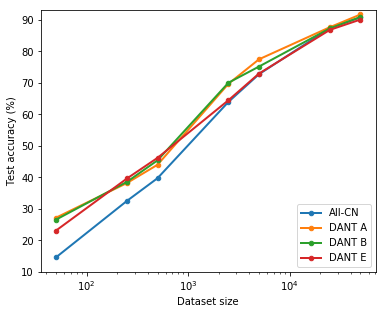
\includegraphics[width=0.31\linewidth]{chapter_7/figures/fig_1.png}
%		%\vspace{-2mm}
%		%\caption{AUC as a function of acquisition step}
%	\end{subfigure}
%	\hfill
%	\begin{subfigure}[]{}
%		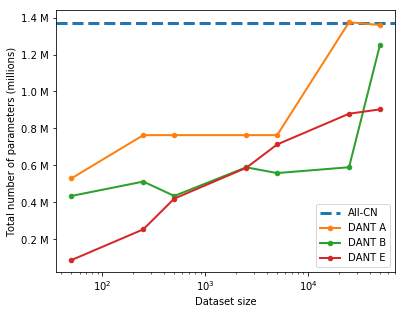
\includegraphics[width=0.32\linewidth]{chapter_7/figures/fig_2.png}
%		%\vspace{-2mm}
%		%\caption{\# of positive examples as a function of acquisition step}
%	\end{subfigure}
%	\hfill
%	\begin{subfigure}[]{}
%		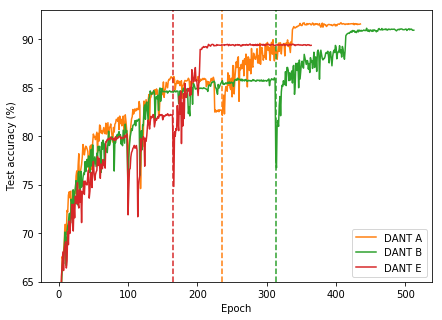
\includegraphics[width=0.33\linewidth]{chapter_7/figures/fig_3.png}
%		%\vspace{-2mm}
%		%\caption{\# of positive examples as a function of acquisition step}
%	\end{subfigure}
%	\vspace{-2mm}
%	\caption{Effect of varying datasize on the performance of discovered models.  }
%	\label{fig:adaptivemodel}
%\end{figure*}

%\begin{figure*}
%% https://tex.stackexchange.com/questions/56163/subfigure-error-missing-number-treated-as-zero
%\centering
%\subfigure[]{}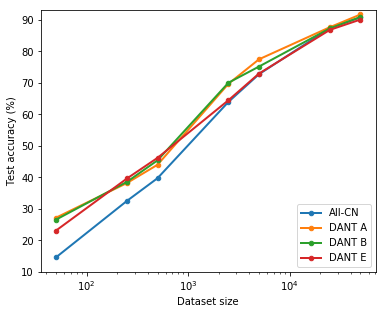
\includegraphics[width=0.4\linewidth]{chapter_7/figures/fig_1.png}
%\subfigure[]{}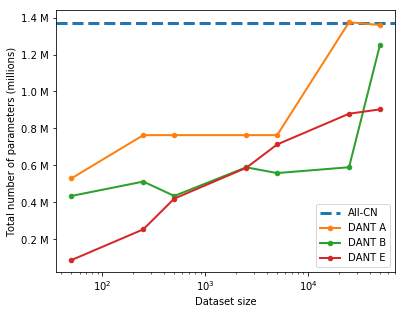
\includegraphics[width=0.4\linewidth]{chapter_7/figures/fig_2.png}
%\caption{Effect of varying datasize on the performance of discovered models.}
%
%\end{figure*}

%%%%%% (backup) Removed result section %%%%%%%%%%
%\subsection{Training time comparison (optional)}
%Tab.\ref{table:traintime} summarise the time taken on a single Titan X GPU for the growth phase and refinement phase of various ANTs, and compare against the training time of All-CN. The local optimisation during the growth phase means that the gradient computation is constrained to the newly added component of the graph, enabling to grow a good candidate model under $2$ hours on a single GPU. 
 
% attains up to $2.5$ times reduction in the required time in comparison with the synthetic experiment where each step of the growth phase is performed via global optimisation. 

 %%%%%% (backup) Removed result section %%%%%%%%%%
% \begin{table}
% 	%\vskip 0.1in  % Was 0.15in
% 	\begin{center}
% 		\begin{small}
% 			%\begin{sc}
% 			\begin{tabular}{l|c|c|c|c}
% 				\hline
% 				\multicolumn{1}{c}{} &  \multicolumn{2}{c}{\textbf{Growth}} & \multicolumn{2}{c}{\textbf{Fine-tune}}  \\
% 				\hline
% 				Model & Time & Epochs  & Time  & Epochs\\
% 				\hline
% %				\abovespace
% %				ANT-MNIST-1  &  &   &LC& 200 \\
% %				ANT-MNIST-2& &  & LC & 200\\
% %				ANT-MNIST-6 & &  &LC & 200 \\
% %				\hline
% 			%	\abovespace
% 				All-CN (baseline)&--~~~ & --~~~ & 1.1 (hr) &200 \\
% 				ANT-CIFAR10-A&1.3 (hr) & 236  & 1.5 (hr) &200 \\
% 				ANT-CIFAR10-B & 0.8 (hr) & 313 & 0.9 (hr) & 200\\
% 				ANT-CIFAR10-C&  0.7 (hr) &  285& 0.8 (hr) & 200 \\
% 				\hline
% 			\end{tabular}
% 			%	\end{sc}
% 		\end{small}
% 	\end{center}
% 	\vspace{-3mm}
% 	\caption{Training time comparison. Time and number of epochs taken for the growth and refinement phase are shown. along with the time required to train the baseline, All-CN.}
% 	\label{table:traintime}
% 	%\vskip 0.1in 
% \end{table}

%\subsection{Representational benefits of split}
%\textcolor{red}{No results yet!}. 
%It would be nice to demonstrate the benefits of splitting over going deeper. I am thinking of growing ANTs but only allowing them to go deeper. We can compare against the standard ANTs which also have the option to split. Hopefully, we get some nice results that quantitatively show the benefits of having an option to partition the data! 

%%%%%% (backup) Removed result section %%%%%%%%%%
%\subsection{Effect of training steps (optional)}
%Number of training steps at each stage in the growth phase affects the discovered architecture, and consequently the classification performance. If too few steps of optimisation are performed, then the added module (additional router or transformer) may simply not be tuned enough. On the other hand, if too many optimisation steps are taken, this causes the added component to overfit. Both extremes prevent the model from making a meaningful further growth. It is therefore important to find the right number of local training steps in order to perform an effective growth phase.

%Some preliminery experiments done. The main point I want to raise here is that underexploration or over-finetuning at local level is bad. You need to find the right amount of time spend at each step of the growth phase to maximize the power of our proposed algorithm. Automating this step is future work. 

% \subsection{EM and stochastic approximation}
% \textcolor{red}{No results yet!}. All the results reported so far are not based on EM. If we have time, it would be nice if we could show that EM performs better than standard back-propagation (not done yet). If not, then we may as well stick to the simpler optimisation algorithm. However, at least we should introduce the stochastic version, which is much lighter weight,  and show how much performance is sacrificed. This may be useful for the community as it may be the key to scale up the method. In the method section, we can briefly draw a connection between this stochastic method and EM, and discuss that one is just an approximation of the other. 

%\textbf{Local optima and weight resetting:} A snippet from S3.2 in \cite{real2017large}: 
%\textit{``the identity mutation offers a mechanism for populations to get trapped in local optima. Some individuals may get trained more than their peers just because they happen to have undergone more identity mutations. It may, therefore, occur that a poor architecture may become more accurate than potentially better architectures that still need more training. In the extreme case, the well-trained poor architecture may become a super-fit individual and take over the population.
%"}